% !TeX root = ncaa-manuscript-en.tex
\section{Proposed Method}\label{sec:method}

GuardSynth makes the evidence and meaning of behavioral constraints explicit,
checks them within supported logical models, and expresses them as language for
learning. It retains the original CoC as a causal explanation of the driving
decision and appends a separately constructed constraint on admissible actions.
The three problems identified in the Introduction organize the method:
construction links fields to evidence, specification checking assesses the
supported logical meaning, and language generation connects that meaning to
learning inputs. Pedestrian entry provides the running example; position
holding extends the admissibility condition to sampled positions over time.

\subsection{Problem Setting}\label{sec:method-problem}

Each example contains a scene input, the original CoC, a set of action candidates
$\mathcal{A}$, and a supplied behavioral rule. A rule is an externally provided
condition; a behavioral constraint makes its applicability, restriction, and
release precise enough to assess admissibility. Supplied rules may represent
experimental policies or operating instructions, so constraint compliance is
distinguished from compliance with traffic laws and regulations.
Let $h_t$ denote the observations and state
history supplied up to decision step $t$. A behavioral constraint $C$ defines
the admissible candidate set
\begin{equation}
A_C(h_t)=\{a\in\mathcal{A}\mid a\text{ satisfies }C\text{ under }h_t\}.
\end{equation}
When several constraints apply, their admissible sets are intersected.
Admissibility here means satisfaction of the stated constraints; physical
feasibility requires the relevant vehicle and environment dynamics to be
modeled as well.

Constraints determine admissibility, whereas the selection objective ranks
admissible candidates. We use the admissible candidate with the greatest
progress score $J(a)$ as the preferred candidate $a^\ast$, whose label is the
reference label used for training and evaluation:
\begin{equation}
a^\ast=\underset{a\in A_C(h_t)}{\arg\max}\;J(a).
\end{equation}
The task generator supplies the synthetic progress score $J(a)$; it is not
part of the logical constraint or an SMT optimization objective. It ranks
candidates for this task rather than measuring distance traveled or long-term
driving efficiency. An admissible choice with a lower score therefore differs
from the preferred candidate without violating the constraint. The
preferred-selection score in Section~\ref{sec:setup-metrics} measures the
frequency of selecting $a^\ast$, rather than the magnitude of a quality loss.

The learning model outputs a label for one of the supplied candidates. Even
when candidate descriptions contain time-indexed coordinates, the model does
not generate a new trajectory. This candidate-selection task differs from the
Alpamayo trajectory-generation diagnostics reported in the Introduction.

\subsection{Workflow}\label{sec:method-workflow}

GuardSynth takes the original CoC, scene observations, supplied rules, and
modeling assumptions through four stages (Fig.~\ref{fig:method-workflow}).
\begin{enumerate}
\item \textbf{Constraint construction:} identify the behavioral restriction and
associate its required information with observations, rules, or assumptions.
\item \textbf{Specification:} represent applicability, restricted actions,
persistence, release, and evidence in an EBLC specification.
\item \textbf{Checking:} inspect the structure and logical interpretation and
compare them with supplied rules and evidence records where supported.
\item \textbf{Language generation:} render the specification as CNL, assess
sentence correspondence where a supported parser is available, and append the
sentences to CoC.
\end{enumerate}
The outputs are an EBLC specification, check records, and sentences for the
learning input. The aim is to maintain correspondence among specification
meaning, check outcomes, and language. Unexpected or UNKNOWN solver outcomes
require review. Structural validation is the renderer's implemented
precondition; logical check outcomes are assessed separately and retained for
review.

\begin{figure}[tbp]
\centering
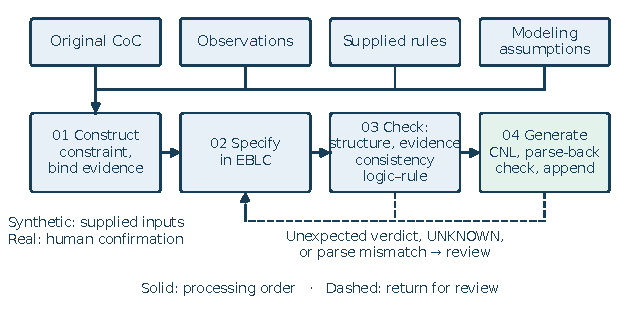
\includegraphics[width=\linewidth]{figures/method-flow.pdf}
\caption{GuardSynth workflow. Four inputs feed four stages. Unexpected
solver verdicts, UNKNOWN, or a sentence-parsing mismatch return the
specification for review. Synthetic experiments use supplied inputs; real
scenes require human confirmation of applicability. In the reported
experiments, evidence and sentence correspondence were assessed after training
(Section~\ref{sec:method-checks}).}
\label{fig:method-workflow}
\end{figure}

\subsection{Constraint Construction and Evidence Binding}\label{sec:method-evidence}

CoC combines observations with a causal explanation; a behavioral constraint
is a separate element that determines which actions are permitted under
specified conditions. A selection objective expresses preferences among
permitted actions.

Constraint construction identifies the applicable situation, the restricted
action, and its bound or release condition. The required information is
associated with one of the three roles in Table~\ref{tab:method-evidence}.

\begin{table}[tbp]
\caption{Roles of information used to construct a constraint}
\label{tab:method-evidence}
\small
\begin{tabularx}{\linewidth}{@{}>{\raggedright\arraybackslash}p{0.19\linewidth}>{\raggedright\arraybackslash}X>{\raggedright\arraybackslash}X@{}}
\toprule
Role & Example & Use in interpretation\\
\midrule
Observation & Time at which the pedestrian leaves the conflict zone & Supplies environmental state and event time\\[3pt]
Supplied rule & Wait at least 0.5 s after clearance & Determines the temporal boundary of admissibility\\[3pt]
Modeling assumption & No reoccupation after clearance & Defines the scope of the temporal interpretation\\
\botrule
\end{tabularx}
\end{table}

This separation distinguishes observed facts from required behavior. Clearance
time can be observed, but the required wait is determined by a separate rule.
Waiting durations and permitted distances are therefore taken from supplied
rules rather than inferred from video or CoC wording.

Conditions and values are linked to their supporting records, as illustrated
in Table~\ref{tab:method-specification}. If a constraint is wrong, these links
identify the observation, rule, or assumption requiring review. Recording a
source does not establish that the source is correct.

In the synthetic experiments, the generator supplies observations, rules, and
candidate measurements to predefined specification constructors. The original
natural-language CoC is retained; these experiments do not parse its unrestricted
meaning into EBLC. Real-scene use requires human confirmation of the
relevant entities, regions, event times, and rule applicability. Automatic
extraction of this information from video and its quality are not evaluated
in this study.

\subsection{EBLC Specifications}\label{sec:method-eblc}

An Evidence-Bound Lifecycle Contract (EBLC) records a behavioral constraint
through its subject and target, applicability, action restriction, persistence
and release, time and units, and supporting evidence and assumptions.
``Evidence-bound'' denotes the connection between values and their source
records. ``Lifecycle'' covers activation, persistence, release, and, where
needed, reactivation. Each task uses the required elements; only combinations
supported by the validator and logical interpretation are accepted.

\noindent\textbf{Pedestrian-entry constraint.}
This constraint prohibits entry while the conflict zone is occupied and
requires a specified wait after clearance. Table~\ref{tab:method-specification}
shows the semantic contents of its specification for a 0.5 s rule and of the
position-hold specification described below, without
implementation identifiers, together with the CNL phrase generated from each
element.

\begin{table}[tbp]
\caption{EBLC specifications and the CNL phrase generated from each element}
\label{tab:method-specification}
\footnotesize
\begin{tabularx}{\linewidth}{@{}>{\raggedright\arraybackslash}p{0.17\linewidth}>{\raggedright\arraybackslash}p{0.24\linewidth}>{\raggedright\arraybackslash}p{0.15\linewidth}>{\raggedright\arraybackslash}X@{}}
\toprule
Element & Value & Role & Generated phrase\\
\midrule
\multicolumn{4}{@{}l}{\textit{Pedestrian entry, 0.5 s wait}}\\[2pt]
Subject and target & Ego vehicle; pedestrian conflict zone & Restriction scope & ``the pedestrian conflict zone''\\[3pt]
Restricted action & No entry during occupancy & Action restriction & ``Do not enter \ldots\ while it is occupied.''\\[3pt]
Release requirement & At least 0.5 s of clearance & Supplied rule & ``Enter only after the zone has remained clear for at least 0.5 s.''\\[3pt]
Assumption & A single clearance transition with no reoccupation & Interpretation scope & Not rendered\\[3pt]
Evidence & Supplied synthetic rule and its source-record identifiers & Traceability & Not rendered\\
\midrule
\multicolumn{4}{@{}l}{\textit{Position hold, 2.0 s}}\\[2pt]
Subject and target & Ego vehicle; initial XY position & Restriction scope & ``the ego vehicle's initial position''\\[3pt]
Hold duration & 2.0 s & Supplied rule & ``Hold \ldots\ for at least 2.0 s.''\\[3pt]
Checked samples & Listed waypoints with $t\le2.0$ s, endpoint included & Interpretation scope & ``At every listed waypoint with t <= 2.0 s, including the endpoint,''\\[3pt]
Restricted action & Radial distance at most 0.2 m & Action restriction & ``the radial XY distance from the initial position must be at most 0.200 m.''\\[3pt]
Release & Motion permitted after the hold & Release & ``Movement after that period is permitted.''\\[3pt]
Assumption & Waypoints relative to the initial origin & Interpretation scope & Stated in candidate descriptions\\[3pt]
Evidence & Supplied synthetic rule and its source-record identifiers & Traceability & Not rendered\\
\botrule
\end{tabularx}
\end{table}

Clearance time is an observation supplied during checking, not a value stored
in this specification. Let $\tau$ be clearance time, $u$ the candidate's entry
time, $\Delta$ the required wait, and $e$ its Boolean entry flag. Under the
no-reoccupation assumption, admissibility requires
\begin{equation}\label{eq:method-entry}
e\Rightarrow u\ge\tau+\Delta.
\end{equation}
The specification supplies $\Delta$, whereas the environment and candidate
supply $\tau$, $u$, and $e$. This separation permits different rules to be
applied to the same environment and different candidates to be checked against
the same specification.

For example, clearance at 11.0 s permits entry from 11.5 s under a 0.5 s rule
and from 12.5 s under a 1.5 s rule. The scene and candidates can be identical
while the admissible set changes. A non-entry candidate satisfies both rules;
its selection depends on progress.

\noindent\textbf{Position-hold constraint.}
This constraint requires a candidate to stay within a permitted radius of its
initial position for a specified duration. Let $T$ be the hold duration, $R$
the permitted radius, and $(x_i,y_i)$ the candidate's sampled coordinates
relative to its initial position. Admissibility requires
\begin{equation}\label{eq:method-hold}
\bigwedge_{t_i\le T}\left(x_i^2+y_i^2\le R^2\right).
\end{equation}
We use $R=0.2\,\mathrm{m}$ and $T\in\{0.5,2.0\}\,\mathrm{s}$. The interval
includes its endpoint; movement after the hold period is unrestricted. Only
the listed samples are checked, rather than continuous motion between samples
or vehicle dynamics.

The same candidates are presented in two forms. \textbf{Time-indexed XY
coordinates} require the model to identify samples within the hold interval
and assess their distances from the initial position. \textbf{Interval maxima}
supply every candidate with both $D_{\max}(0.5\,\mathrm{s})$ and
$D_{\max}(2.0\,\mathrm{s})$, where
$D_{\max}(T)=\max_{t_i\le T}\sqrt{x_i^2+y_i^2}$, regardless of the active
rule; the model must still select the required interval and compare its
maximum with the permitted radius. Reference admissibility is computed from
the original integer coordinates and squared distances, not rounded maxima
displayed in the prompt. Comparing the two forms helps distinguish
coordinate-calculation demands from constraint-based selection, although it
also changes the input representation.

\noindent\textbf{Numerical bounds.}
Speed, clearance, and entry-delay tasks place an upper or lower bound on a
candidate measurement. With completion flag $q$, measurement $x$, and bound
$b$, the basic form is
\begin{equation}
q\Rightarrow(x\ \mathrm{op}\ b),\qquad
\mathrm{op}\in\{\le,\ge\}.
\end{equation}
Section~\ref{sec:method-cnl} explains the treatment of non-completing
candidates and its difference from the generated language.

\noindent\textbf{Activation, persistence, and release.}
The preceding constraints are evaluated from supplied values. A separate
qualitative specification tracks obligations when evidence changes over time:
valid activation or release evidence updates the state, while uncertain or
conflicting evidence preserves the previous state. Its state-transition checks
are reported in Supplementary Section S3; the learning experiments
do not use this specification.

Table~\ref{tab:method-tasks} connects each task to its admissibility condition.
The first six tasks form the six-task comparison; position holding is evaluated
in both the fresh-adapter and continuation studies. All numerical bounds are
supplied experimental rules. Entry delay $\delta$ is a duration, whereas $u$ is an instant. In stopping,
$o$ is position relative to the stop line, with negative values before the
line; $a_{\mathrm{peak}}$ and $j_{\mathrm{peak}}$ denote peak deceleration and jerk.

\begin{table}[tbp]
\caption{Task admissibility conditions with representative supplied rules.
$q$ denotes completion and $e$ denotes entry.}
\label{tab:method-tasks}
\small
\begin{tabularx}{\linewidth}{@{}>{\raggedright\arraybackslash}p{0.22\linewidth}>{\raggedright\arraybackslash}X@{}}
\toprule
Task & Admissibility condition\\
\midrule
Maximum speed & $q\Rightarrow v\le4.4\,\mathrm{m/s}$\\[4pt]
Minimum clearance & $q\Rightarrow d\ge2.0\,\mathrm{m}$\\[4pt]
Minimum entry delay & $q\Rightarrow\delta\ge2.5\,\mathrm{s}$\\[4pt]
Pedestrian entry & $e\Rightarrow u\ge\tau+\Delta$\\[4pt]
Stopping & $q\Rightarrow(o\le0\land a_{\mathrm{peak}}\le5.8\,\mathrm{m/s^2}\land j_{\mathrm{peak}}\le7.4\,\mathrm{m/s^3})$\\[4pt]
Lane change & $q\Rightarrow g\ge5.8\,\mathrm{m}$\\[4pt]
Position holding & $\displaystyle\bigwedge_{t_i\le T}(x_i^2+y_i^2\le R^2)$\\
\botrule
\end{tabularx}
\end{table}

\subsection{Specification Checking}\label{sec:method-checks}

The admissibility conditions in Section~\ref{sec:method-eblc} are translated
into logical formulas. We use SMT and
Z3~\cite{r11,r12} and distinguish property queries from candidate queries.
The learning specifications are evaluated through satisfiability, candidate
admissibility, and concrete logic--rule comparisons. Property-query semantics
are illustrated below; the separate qualitative lifecycle example in
Supplementary Section S3 is not used for learning.

\noindent\textbf{Specification properties.}
Let $\Phi$ combine the specification and its assumptions, and let $P$ be a
property of interest. The counterexample query is
\begin{equation}
\Phi\land\neg P.
\end{equation}
UNSAT means that no counterexample exists within the encoded scope. SAT means
that an assignment satisfies the specification while violating the property.
Because an inconsistent specification implies every property vacuously, the
satisfiability of $\Phi$ is checked separately.

For the entry constraint, the requirement that entry occur only after the
release boundary can be expressed as $P=(e\Rightarrow u\ge\tau+\Delta)$.
Its counterexample query, $\Phi_C\land e\land(u<\tau+\Delta)$, must be UNSAT.
Removing the release restriction permits a SAT counterexample. This illustrates
property-query semantics; the fault-injection logic--rule comparisons below use
concrete boundary assignments.

\noindent\textbf{Candidate queries.}
Let $B(a)$ fix candidate $a$'s measurements and completion or entry flag. We
check
\begin{equation}
\Phi_C\land B(a).
\end{equation}
SAT means that the candidate is compatible with the constraint, and UNSAT means
that it is incompatible. This query checks admissibility, not whether the
candidate is the preferred one.

Before training, the pedestrian-entry and position-hold specifications used for
learning underwent structural validation, satisfiability checks, and candidate
checks.

\noindent\textbf{Checking layers.}
Five checks compare different objects.
\begin{enumerate}
\item \textbf{Structural check:} verify supported field combinations, values,
and units.
\item \textbf{Satisfiability check:} confirm that the base specification is
satisfiable, so that properties do not hold vacuously.
\item \textbf{Logic--rule comparison:} compare logical verdicts for concrete
candidates with verdicts computed by independent integer rules from the
supplied rule. Archived action candidates are evaluated together with boundary
probes: for pedestrian entry, entry or non-entry at $-1,0,+1$ ms around release;
for position holding, distances of 199, 200, and 201 mm, with diagonal norm
checks, at every listed non-initial sample, including samples after release.
The 1 ms spacing tests logical boundaries, not vehicle-control precision.
\item \textbf{Evidence correspondence check:} compare the specification with
the supplied rule record.
\item \textbf{Sentence correspondence check:} parse the generated CNL with a
fixed grammar for the specification, reconstruct the supported fields, and
compare them with the original specification.
\end{enumerate}
Evidence correspondence, sentence correspondence, and boundary probes for
logic--rule comparison were added for the fault-injection evaluation below;
they were not applied in the reported training runs.

\noindent\textbf{Fault-injection evaluation.}
To assess which check detects which error, we inject faults into the
pedestrian-entry and position-hold specifications used to produce learning
inputs. Each task contributes 24 base cases: 12 archived evaluation contexts
paired with two supported durations (0.5/1.5 s for entry and 0.5/2.0 s for
holding). These are repeated contexts under two rule settings, not 24 distinct
specification parameterizations or independent road scenes. Before injection,
we verify the archived specifications and P2 text against the maintained
constructors and renderers. The evaluation reuses the unaltered structural
validators, logical lowering, renderers, and SMT compiler.

Each base case yields one valid case, six supported faults, and one control in
which the source record and the specification are changed to the same wrong
value: 192 cases per task and 384 in total. The faults change a supported
duration in the specification only, reverse a comparison, omit a release
condition, change a unit without rescaling, or alter the sentence's duration
or negation. For entry, release omission removes the entry gate. For holding,
it keeps the distance restriction active after the hold ends, and comparison
reversal affects the inclusive hold endpoint. The probes comprise 7,392
concrete queries; UNKNOWN outcomes are recorded separately. Detection results
are reported in Section~\ref{sec:results-checks} (Table~\ref{tab:results-faults}).

Sentence correspondence is limited to each specification's fixed grammar.
Fixed patterns constrain the target, units, negation, and relation; the parser
extracts the duration and reconstructs the supported fields. This is not a
general test of semantic equivalence for arbitrary language. An earlier
fault-injection evaluation on a separate pedestrian-entry specification,
developed for the expression-diversity study, uses probes at $-100,0,+100$ ms
(192 cases) and is described in Supplementary Section S4.

\noindent\textbf{Scope of the checks.}
Check conclusions hold only within supported specification structures,
supplied inputs, explicit assumptions, and the finite logical scope. The
accident examples in the Introduction motivate checking interacting
requirements, but the reported experiments assess the supported task
specifications rather than reconstructing those accidents or verifying a
general composition of traffic rules and vehicle dynamics. Consistency of a
specification alone does not establish safe behavior or progress toward an
objective. Pedestrian entry assumes a single clearance transition without
reoccupation; position holding checks only listed coordinate samples.
Evidence records and internal consistency do not establish observation truth,
rule suitability, or road safety, and logic--rule comparison establishes
correspondence between two implementations of the same supplied rule.

Specification checking and model evaluation measure different objects. The
former assesses correspondence among structure, evidence, logic, and language;
the latter measures whether the selected candidate is admissible and
preferred. A model can select a prohibited candidate even when its
specification passes the checks, so Section~\ref{sec:results} reports the two
with their respective evaluation units and denominators.

\subsection{Composition of Supplied Constraints}\label{sec:method-composition}

The composition diagnostic checks whether separately supplied conditions can
hold together under an explicit shared context. Let $\Phi_E$ encode supplied
observations and modeling assumptions, and let $\Phi_j$ encode source
constraint $j$. For a selected source set $\Gamma$, the query is
\begin{equation}
\Phi_E\land\bigwedge_{j\in\Gamma}\Phi_j.
\end{equation}
SAT provides an assignment satisfying the selected conditions together;
UNSAT identifies an incompatible combination relative to $\Phi_E$. The context
is checked first. Every source constraint is then checked separately, in pairs,
and in the full combination. Enumerating subsets for these two- or three-source
cases identifies subset-minimal conflict groups: the group is UNSAT and every
proper subset is SAT. This identifies incompatible requirements, not which
source should be changed.

Documented conditions are kept separate from authored states, candidate
requests, modeling assumptions, and test objectives. We manually reviewed
official accident investigations, operating guides, traffic guidance, and
regulations; the selected cases use NTSB, FHWA, Waymo, and UK Department for
Transport documents. The constraints are manually formalized, then executed
by the unchanged platform Core/SMT compiler. Supplementary Section S13 lists every natural-language statement
with its source role and formal condition; these statements explain the
formalization and are not outputs of an unrestricted parser or the CNL
correspondence evaluation.

The braking case selects the historical suppression branch with an already
recognized emergency, persistent hazard, no takeover, and no alternative
path~\cite{NTSB2019Tempe}. The NTSB policy record gives a braking delay
$t_b\ge1$ s; an authored constant-deceleration model gives stopping distance
$x\ge vt_b+v^2/(2a)$; and an authored test objective requires $x\le d$.
Emergency-trigger eligibility and jerk are outside the model, and the
authored terms determine whether the selected delay is compatible with a
hypothetical state. The signal case uses FHWA's nominal stopping
model and a two-action stop/proceed abstraction~\cite{FHWA2009Yellow,FHWA2008Timing}.
The interlock case checks candidate autonomous driving against the
manufacturer's listed blockers~\cite{Waymo2026Emergency}; it makes no claim
about rolling or towing. The Rule 129 case fixes other exceptions absent
and compares a restricted faithful encoding with a deliberately omitted
stationary-vehicle exception~\cite{DfT2015HighwayCode129}.

Candidate requests are explicit: permission to cross does not require
crossing, and a blocked driving candidate does not make holding inconsistent.
These distinctions prevent manufactured conflicts from turning optional
progress into an unconditional obligation. The diagnostic checks
compatibility within the stated abstractions, rather than reconstructing
accidents or establishing the safety of an operating system or a complete
operating policy. Supplementary Section S13 retains the earlier synthetic
boundary diagnostic separately.

\subsection{Language Generation and CoC Augmentation}\label{sec:method-cnl}

CNL is generated only from structurally validated specifications. Fixed
sentence rules express the target, restricted action, condition, value, and
unit. Neither reference labels nor progress scores are inputs to the renderer.
The pedestrian-entry specification with a 0.5 s wait generates:
\begin{quote}\small
Do not enter the pedestrian conflict zone while it is occupied. Enter only
after the zone has remained clear for at least 0.5 s.
\end{quote}
The first sentence expresses the occupancy prohibition; the second expresses
the release and waiting condition (Table~\ref{tab:method-specification}). ``At least''
includes the boundary, and ``only after'' states a necessary condition for
entry rather than an instruction to enter at a particular time.
Generated sentences follow the original CoC, before candidate descriptions and
the selection instruction. Fig.~\ref{fig:method-inputs} reproduces two complete
model inputs. Clearance time is supplied separately, so this text does not give the answer
time directly. The EBLC specification, check verdicts, and evidence records
are not inserted into the model prompt.

\begin{figure}[tbp]
\centering
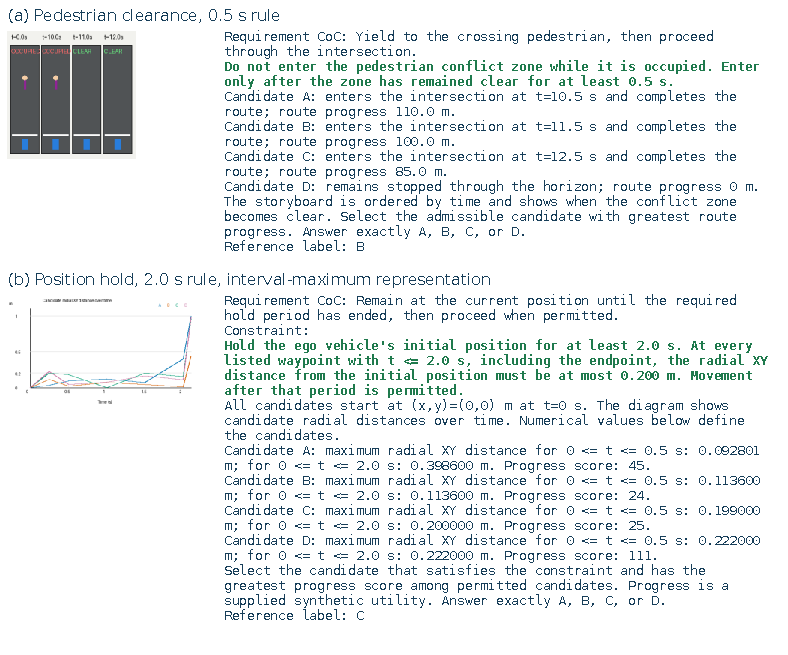
\includegraphics[width=\linewidth]{figures/input-examples.pdf}
\caption{Two archived test inputs. (a) Pedestrian entry with a 0.5 s rule.
(b) Position hold with a 2.0 s rule and interval-maximum candidate
descriptions. Bold green text is the CNL generated from an EBLC specification
(P2); P0 inputs omit it. Text is verbatim except for line breaks added around
the CNL. The model outputs one candidate label; the reference label is shown
for illustration and is not part of the input.}
\label{fig:method-inputs}
\end{figure}

\noindent\textbf{Comparison conditions.}
P0 uses the original CoC, P1 adds a directly written natural-language guard,
and P2 adds CNL generated from an EBLC specification. For pedestrian entry, P1 uses a
template from the preceding study that produces language directly from rule
values~\cite{r4}:
\begin{quote}\small
Do not enter while the pedestrian conflict zone is occupied. After it becomes
clear, remain stopped for at least 0.5 s before entering.
\end{quote}
The temporal candidates specify entry times or non-entry, so P1 and P2 induce
the same admissible set in this task. However, ``remain stopped'' is stronger:
it also restricts motion without entry. We do not claim equivalence for general
trajectories.

For position holding, the original CoC is:
\begin{quote}\small
Remain at the current position until the required hold period has ended, then
proceed when permitted.
\end{quote}
Its P1 natural-language guard uses a template written for this task:
\begin{quote}\small
For the first 2.0 seconds, keep the vehicle within 0.200 metres of its starting
point at all listed times, including the final time of this waiting period.
Moving farther away is allowed only after this period ends.
\end{quote}
Its P2 sentences are generated from the position-hold specification
(Table~\ref{tab:method-specification}; Fig.~\ref{fig:method-inputs}b).
P1 and P2 share a learning interface; their comparison examines differences
in wording and construction path. Rule availability in each study is
summarized in Table~\ref{tab:setup-comparisons}.

\noindent\textbf{Scope of sentence correspondence.}
The logical conditions for static and maneuver tasks do not classify
non-completing candidates as violations, but their generated sentences do not
express this exemption. Sentence--logic correspondence in these tasks is
therefore limited to numerical bounds for completing candidates.

% project_id: guardsynth-coc
\noindent\textbf{Use of AI-assisted tools.}
OpenAI Codex was used to assist with English translation and revision of the
manuscript and with implementation and checking of supporting scripts. The
authors retain responsibility for the scientific content, analyses, and final
manuscript. This assistance is separate from the Qwen and Alpamayo models
evaluated in the experiments.

